\documentclass[11pt]{article}

\usepackage[brazilian]{babel}
\usepackage[utf8]{inputenc}
\usepackage[T1]{fontenc}

\usepackage{graphicx}
\usepackage{subfig}

\usepackage{amsmath}
\usepackage{algorithm}
\usepackage[noend]{algpseudocode}

\title{\textbf{Algoritmo Genético - Problema da Mochila}}

\author{André Minoro Fusioka}

\date{}
\begin{document}

\maketitle

\section{Penalização}

A penalização foi alterada em relação ao apresentado no primeiro relatório individual. Para a penalização de indivíduos da populção avaliada, foi adotada a seguinte métrica: 
$$
fitness\_ajustado(x_n) =
\begin{cases}
 fitness(x_n) & \text{ se } peso(x_n) \leq  C \\ 
 log(peso(x_n)) & \text{ se } peso(x_n) >  C 
\end{cases}
$$
onde $fitness\_ajustado$ é o valor do fitness após a penalização, os valores mais altos são selecionados para a próxima geração. O $peso(x_n)$ é a soma do peso de todos os itens na mochila do n-ésimo indivíduo.

O código abaixo ilustra o cálculo:

\begin{algorithm}
	\caption{Fitness Ajustada}\label{euclid}
	\begin{algorithmic}[1]
		\Function{FitnessAjustada}{população}
		
			\State $fitness\_ajustado \gets []$
			
			\Loop { $\forall$ $individuo$ da $população$:}
				 \State $peso \gets calcular\_peso(individuo)$
				\If{$peso < C$}
				
					\State $fitness \gets calcular\_fitness(individuo) $
				 \Else
					\State $fitness \gets log(peso)$		 
				\EndIf
				\State \textbf{adicione} o $fitness$ à lista $fitness\_ajustado$
			\EndLoop {\textbf{end loop}}
			\State \Return $fitness\_ajustado$
		\EndFunction
	\end{algorithmic}
\end{algorithm}

Cada indivíduo tem o seu peso calculado, se estiver abaixo do limite o fitness real é adicionado à lista de fitness ajustado (sem realizar operação nenhuma), caso esteja acima do limite o fitness penalizado será calculado conforme descrito e então adicionado à lista de fintess ajustado. 

\section{Reparação}

A reparação não sofreu alteração em relação ao primeiro relatório entregue. Para a reparação o peso de cada mochila de cada indivíduo é avaliado e enquanto for maior que o limite um item aleatório é retirado. Quando o peso estiver dentro do limite o fitness dessa mochila é avaliada e adicionada a lista de fintess reparada. O pseudocódigo é exibido abaixo: 


\begin{algorithm}
	\caption{Fitness Reparado}\label{euclid}
	\begin{algorithmic}[1]
		\Function{FitnessReparado}{população}
		
			\State $fitness\_reparado \gets []$
			
			\Loop{ $\forall$ $individuo$ da $população$:}
				\State $peso \gets calcular\_peso(individuo)$
				
				\Loop{ \textbf{enquanto} $peso$ > $C$}
					\State $ individuo \gets remove\_item\_aleatorio(individuo) $
					\State $peso \gets calcular\_peso(individuo)$
				\EndLoop{\textbf{end loop}}
				
				
				\State \textbf{adicione} o $fitness$ à lista $fitness\_reparado$
			\EndLoop{\textbf{end loop}}
			\State \Return $fitness\_reparado$
		\EndFunction
	\end{algorithmic}
\end{algorithm}

Dessa forma, caso os itens da mochila do indivíduo estejam dentro do limite permitido seu fitness é adicionado à lista de fintess reparados (sem realizar operação nenhuma), caso esteja acima do limite um item aleatório é removido da mochila até estar dentro do limite, quando estiver dentro do limite seu fitness é calculado e adicionado à solução.

\section{Penalização x Reparação}

A implementação da penalização foi alterada em relação ao primeiro relatório. A  \ref{fig:comparacao} exibe média dos fitness encontrados na implementação nova e na implmentação antiga.

A curva vermelha representa a penalização e a curva azul representa a reparação. Possível notar que a curva azul permanece acima da curva vermelha, mostrando que a reparação obteve resultados melhores.

Também é notável que a nova implementação da reparação apresentada na Figura \ref{fig:ag_comparacao_100_500_09_01}, representada pela curva vermelha, tem um crescimento muito mais suave se comparado com a implementação antiga da Figura \ref{fig:comparacao_100_500_08_005}.

\begin{figure}[h]
	\centering
	\subfloat[Nova implementação de penalização]{
		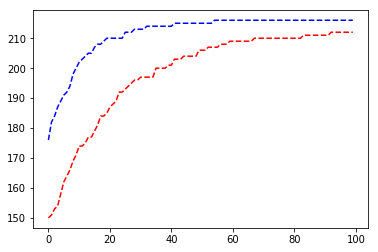
\includegraphics[scale=0.4]{./saida/ag_100_500_08_005.png}
		\label{fig:ag_comparacao_100_500_09_01}
	}
	\quad %espaco separador
	\subfloat[Implmentação antiga de penalização]{
		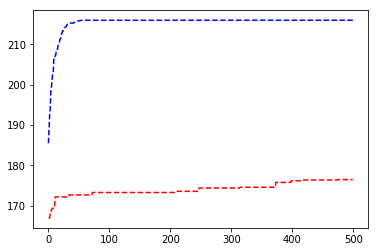
\includegraphics[scale=0.4]{ag_comparacao_500_500_08_005.png}
		\label{fig:comparacao_100_500_08_005}
	}
	\caption{Gráficos de comparação entre as abordagens de penalização e reparação da implementação nova e antiga}
	\label{fig:comparacao}
\end{figure}



Em todos os casos o comportamento a reparação se mostrou superior, enquanto subindo rápidamente para um valor ótimo, enquanto a penalização teve um crescimento mais lento, com uma melhora lenta e inferior à reparação.


\section{Soluções encontradas}

Todos os testes foram executados dez vezes, com um número máximo de 500 gerações.

A melhor mochila encontrada na reparação obteve o fitness de 216:

< 13, 120, 216, 0, 0, 0, 1, 0, 0, 0, 1, 1, 1, 0, 0, 0, 0, 1, 0, 0, 1, 1, 0, 0, 0, 0, 0, 0, 0, 0, 0, 1, 1, 0, 0, 0, 1, 0, 0, 0, 1, 0, 1, 0, 1 > 

< 14, 120, 216, 0, 0, 0, 1, 0, 0, 0, 0, 1, 1, 0, 0, 0, 0, 1, 0, 0, 1, 1, 0, 0, 1, 0, 1, 0, 0, 0, 0, 1, 1, 0, 0, 0, 1, 0, 0, 0, 1, 0, 1, 0, 1 > 


Já a implementação de penalização obteve como melhor fitness o valor de 215, apesar de não chegar ao mesmo resultado da reparação houve uma grande melhora em comparação com a implementação feita para o primeiro relatório. Sendo as configurações de mochila com o fintess máximo as seguintes: 

< 13, 119, 215, 0, 0, 0, 1, 0, 0, 0, 0, 1, 0, 0, 0, 0, 0, 1, 0, 0, 1, 1, 0, 0, 1, 0, 1, 0, 0, 0, 0, 1, 1, 0, 0, 0, 1, 0, 0, 0, 1, 0, 1, 0, 1 > 

< 12, 119, 215, 0, 0, 0, 1, 0, 0, 0, 1, 1, 0, 0, 0, 0, 0, 1, 0, 0, 1, 1, 0, 0, 0, 0, 0, 0, 0, 0, 0, 1, 1, 0, 0, 0, 1, 0, 0, 0, 1, 0, 1, 0, 1 > 

Todas as saídas podem ser vistas em: https://github.com/Minoro/data-science-theory/tree/master/IA


\section{Comparação de Cálculo de Fitness}

Para as análises a seguir assume-se a função fitness como sendo apenas a soma dos valores dos itens da mochila, e também que é permitido a geração de uma população inicial com indivíduos infactíveis, sendo assim a penalização e reparação também devem ser aplicados aos pais.

Para a solução de penalização o cálculo de fitness é realizado na seleção por roleta para a primeira geração e durante a penalização para cada pai e filho que estiver dentro do peso limite, pois caso seja penalizado o valor da mochila não é levado em consideração, apenas seu peso. Nesse caso em que a soma dos pesos não está sendo considerada para a análise, temos:

\begin{equation} \label{eq:complexidade_pelanizacao}
	O(n) = Np_{pais} + Np_{filhos}
\end{equation}

Ou seja, duas vezes para cada indivíduo de uma geração, sendo $Np_{pais}$ para os pais e $Np_{filhos}$ para os filhos, como o número de pais é igual ao número de filhos temos $2Np$.

Já para a abordagem de reparação temos a avaliação fitness realizada para os pais e para cada indivíduo da população (pais e filho) que passe do peso é necessário calcular mais uma vez mais uma vez.

Dessa forma temos:
\begin{equation} \label{eq:complexidade_reparacao}
	O(n) = Np_{pais} + Np_{pais} + Np_{filhos} = 3Np
\end{equation}

Dessa forma,temos que o cálculo da penalização é mais eficiente, pois há chances que não aplicar o cálculo de fitness a todos os indivíduos utilizando o cálculo feito para a roleta.


\end{document}
